%!TEX program = xelatex
% 完整编译: xelatex -> biber/bibtex -> xelatex -> xelatex
\documentclass[lang=cn,11pt,a4paper]{paper}

\title{编译原理与技术 实验一:词法分析程序的设计与实现 \\ 实验报告}
\author{张梓良 \\ 2021212484}
\institute{北京邮电大学 \\ 计算机科学与技术}

\date{\zhtoday}


% 本文档命令
\usepackage{array}
\newcommand{\ccr}[1]{\makecell{{\color{#1}\rule{1cm}{1cm}}}}
\usepackage{xcolor}
% 定义可能使用到的颜色
\definecolor{CPPLight}  {HTML} {686868}
\definecolor{CPPSteel}  {HTML} {888888}
\definecolor{CPPDark}   {HTML} {262626}
\definecolor{CPPBlue}   {HTML} {4172A3}
\definecolor{CPPGreen}  {HTML} {487818}
\definecolor{CPPBrown}  {HTML} {A07040}
\definecolor{CPPRed}    {HTML} {AD4D3A}
\definecolor{CPPViolet} {HTML} {7040A0}
\definecolor{CPPGray}  {HTML} {B8B8B8}
\lstset{
    columns=fixed,       
    numbers=left,                                        % 在左侧显示行号
    frame=none,                                          % 不显示背景边框
    backgroundcolor=\color[RGB]{245,245,244},            % 设定背景颜色
    keywordstyle=\color[RGB]{40,40,255},                 % 设定关键字颜色
    numberstyle=\footnotesize\color{darkgray},           % 设定行号格式
    commentstyle=\it\color[RGB]{0,96,96},                % 设置代码注释的格式
    stringstyle=\rmfamily\slshape\color[RGB]{128,0,0},   % 设置字符串格式
    showstringspaces=false,                              % 不显示字符串中的空格
    language=c++,                                        % 设置语言
    morekeywords={alignas,continute,friend,register,true,alignof,decltype,goto,
    reinterpret_cast,try,asm,defult,if,return,typedef,auto,delete,inline,short,
    typeid,bool,do,int,signed,typename,break,double,long,sizeof,union,case,
    dynamic_cast,mutable,static,unsigned,catch,else,namespace,static_assert,using,
    char,enum,new,static_cast,virtual,char16_t,char32_t,explict,noexcept,struct,
    void,export,nullptr,switch,volatile,class,extern,operator,template,wchar_t,
    const,false,private,this,while,constexpr,float,protected,thread_local,
    const_cast,for,public,throw,std},
    emph={map,set,multimap,multiset,unordered_map,unordered_set,
    unordered_multiset,unordered_multimap,vector,string,list,deque,
    array,stack,forwared_list,iostream,memory,shared_ptr,unique_ptr,
    random,bitset,ostream,istream,cout,cin,endl,move,default_random_engine,
    uniform_int_distribution,iterator,algorithm,functional,bing,numeric,},
    emphstyle=\color{CPPViolet}, 
}

\begin{document}

\maketitle

\section{概述}

\subsection{实验内容及要求}

\begin{enumerate}
  \item 选定源语言,比如:\ \lstinline{C、Pascal、Python、Java}\ 等,任何一种语言均可。
  \item 可以识别出用源语言编写的源程序中的每个单词符号,并以记号的形式输出每个单词符号。
  \item 可以识别并跳过源程序中的注释。
  \item 可以统计源程序中的语句行数、各类单词的个数、以及字符总数,并输出统计结果。
  \item 检查源程序中存在的词法错误,并报告错误所在的位置。
  \item 对源程序中出现的错误进行适当的恢复,使词法分析可以继续进行,对源程序进行一次扫描,即可检查并报告源程序中存在的所有词法错误。
\end{enumerate}

\subsection{实验环境}

\begin{itemize}
    \item cmake version 3.27.0-rc4
    \item gcc version 8.1.0
    \item Visual Studio Code 1.82.2
    \item OS: Windows\_NT x64 10.0.22621
\end{itemize}

\subsection{实验目的}

采用\ \lstinline{C++}\ 作为实现语言,手工编写一个\ \lstinline{C}\ 语言的词法分析程序。

\section{程序设计说明}

\subsection{模块划分}

词法分析程序分为四个模块:\lstinline{token, lexical_analysis, output, main}\ ,其中\ \lstinline{token}\ 模块定义了所需的数据结构,\ \lstinline{lexical_analysis}\ 模块对读入的源程序文件流进行词法分析,\ \lstinline{output}\ 模块将词法分析得到结果输出,\ \lstinline{main}\ 模块将前三个模块组装构成整个词法分析程序。模块间的调用关系如\ \textbf{图\ \ref{fig:模块调用关系}}\ 。

\begin{figure}[!htb]
    \centering
    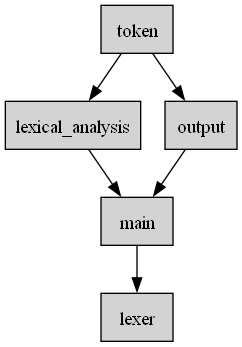
\includegraphics[
    width=0.3\textwidth]{module.png}
    \caption{模块调用关系}
    \label{fig:模块调用关系}
\end{figure}

\subsection{自定义数据结构}

\subsubsection{C语言记号类型}

\begin{lstlisting}
enum TokenType
{
    KEYWORD,              // 关键字
    ID,                   // 标志符
    STRING,               // 字符串常量
    CHAR,                 // 字符常量
    INT,                  // 整型常量
    UINT,                 // 无符号整型常量
    LONG,                 // 长整型常量
    ULONG,                // 无符号长整型
    LONGLONG,             // 长长整型常量
    ULONGLONG,            // 无符号长长整型常量
    FLOAT,                // 单精度浮点数
    DOUBLE,               // 双精度浮点数
    LONGDOUBLE,           // 长双精度浮点数
    RELATION_OPERATOR,    // 关系运算符
    ASSIGN_OPERATOR,      // 赋值运算符
    AGORITHM_OPERATOR,    // 算术运算符
    LOGICAL_OPERATOR,     // 逻辑运算符
    BITWISE_OPERATOR,     // 位运算符
    QUESTION_MARK,        //"?"
    COLON,                //":"
    SEMICOLON,            //";"
    LEFT_SQUARE_BRACKET,  //"["
    RIGHT_SQUARE_BRACKET, //"]"
    LEFT_PARENTHESE,      //"("
    RIGHT_PARENTHESE,     //")"
    LEFT_BRACE,           //"{"
    RIGHT_BRACE,          //"}"
    DOT,                  //"."
    COMMA,                //","
    ARROW,                //"->"
    ANNOTATION,           // 注释
};
\end{lstlisting}

采用\ \lstinline{enum}\ 类型存储记号类型,建立记号类型与非负整数之间的映射,便于词法分析时函数之间记号类型的传递。

\subsubsection{记号属性类型}

\begin{lstlisting}
union ValueType
{
    char charValue;
    int intValue;
    unsigned int uintValue;
    long longValue;
    unsigned long ulongValue;
    long long longlongValue;
    unsigned long long ulonglongValue;
    float floatValue;
    double doubleValue;
    long double longdoubleValue;
};
\end{lstlisting}

考虑到记号的属性类型可能为多种,eg.\ \lstinline{int, char...},因此采用\ \lstinline{union}\ 来定义属性类型。同时当属性值为字符串时,由于字符串的大小不定,所以采用存储字符串在相应字符串表中的下标\ \lstinline{index}\ 来间接访问字符串。

\subsubsection{记号}

\begin{lstlisting}
struct Token
{
    TokenType type;  // 记号类型
    ValueType value; // 记号值
    int line;        // 记号所在行数
    int column;      // 记号所在列数
};
\end{lstlisting}

一个记号中存储了记号类型、记号属性值、记号所在行数以及记号所在列数,其中记号类型和记号属性值采用先前已经自定义的数据类型。记号的表示形式为\ \lstinline{<line:column><type, value>}\ 。

\subsubsection{C语言关键字}

\begin{lstlisting}
const vector<string> KeyWord = {
    "auto", "break", "case", "char", "const", "continue", "default", "do", "double",
    "else", "enum", "extern", "float", "for", "goto", "if", "inline", "int", "long",
    "register", "restrict", "return", "short", "signed", "sizeof", "static", "struct",
    "switch", "typedef", "union", "unsigned", "void", "volatile", "while", "_Bool",
    "_Complex", "_Imaginary"};
\end{lstlisting}

参考\ \lstinline{ISO\_C99\_definition}\ 中对关键字的定义:\ \textbf{图\ \ref{fig:C99对关键字的规定}}\ ,将C语言中所有关键字存储在一个\ \lstinline{vector}\ 容器中。类型为关键字的记号可以通过相应下标索引在\ \lstinline{KeyWord}\ 表中查找到对应的属性值。

\begin{figure}[!htb]
    \centering
    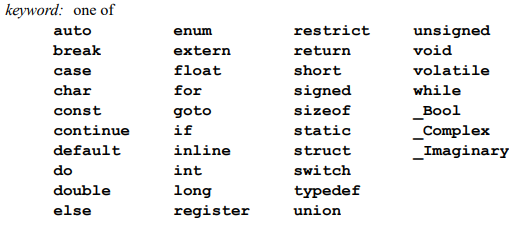
\includegraphics[
    width=0.7\textwidth]{keyword_def.png}
    \caption{C99对关键字的规定}
    \label{fig:C99对关键字的规定}
\end{figure}

\subsubsection{C语言运算符}

\begin{lstlisting}
const vector<string> Operator = {
    "+", "-", "*", "/", "%", "++", "--", "&&", "||", "!", "&", "|", "~", "^", "<<",
    ">>", "=", "+=", "-=", "*=", "/=", "%=", "&=", "|=", "^=", "<<=", ">>=", "==",
    "!=", ">", "<", ">=", "<="};
\end{lstlisting}

由于在记号类型的定义中将运算符分为了五大类\ \lstinline{RELATION_OPERATOR, ASSIGN_OPERATOR, AGORITHM_OPERATOR, LOGICAL_OPERATOR, BITWISE_OPERATOR}\ ,这五大类下又包括若干相应的运算符。所以应存储下所有的运算符,使得类型为运算符的记号可以通过下标索引在\ \lstinline{Operator}\ 表中查找到对应的属性值。

\subsection{词法分析}
词法分析主要由\ \lstinline{lexical_analysis.h}\ 中定义的函数\ \lstinline{lexical_analysis}\ 完成。

\begin{lstlisting}
/**
 * @brief 词法分析
 * 
 * @param fin 输入文件流 
 * @param char_num 读入字符数
 * @param line 当前行数
 * @param col 当前列数
 * @param token_streams 记号流
 * @param id_table 标识符表
 * @param str_table 字符串表
 */
void lexical_analysis(ifstream &fin, int &char_num, int &line, int &col, vector<Token> &token_streams, vector<string> &id_table, vector<string> &str_table);
\end{lstlisting}

该函数设计的核心思想是将识别各类记号的\ \lstinline{DFA}\ 用代码实现。

\subsubsection{设计流程}

参考\ \lstinline{ISO_C99_definition}\ 中对各类记号的形式化定义画出识别各类记号的\ \lstinline{DFA}\ ,再采用\ \lstinline{dot}\ 语言在电脑中绘制出\ \lstinline{png}\ 格式的\ \lstinline{DFA}\ 状态转移图, 最会根据状态转移图编写相应\ \lstinline{C++}\ 程序。

用\ \lstinline{C++}\ 的\ \lstinline{case}\ 语句实现\ \lstinline{DFA}\ ,每一个\ \lstinline{case}\ 对应\ \lstinline{DFA}\ 中的一个状态,\lstinline{cases}\ 之间的跳转对应 \ \lstinline{DFA}\ 中相应状态间的转换。

\subsubsection{标识符或关键字的识别}

\ \lstinline{ISO_C99_definition}\ 中对标志符的定义如\ \textbf{图\ \ref{fig:C99对标识符的规定}}\ 所示。标识符只能由\ \lstinline{_ \ letter}\ 开头,可以包含\ \lstinline{_ \ letter \ digit}\ 。

\begin{figure}[!htb]
    \centering
    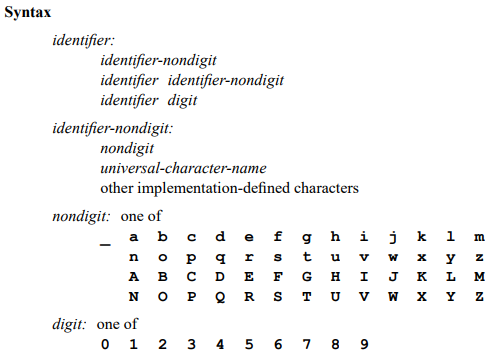
\includegraphics[
    width=0.7\textwidth]{identifier_def.png}
    \caption{C99对标识符的规定}
    \label{fig:C99对标识符的规定}
\end{figure}

采用\ \lstinline{dot}\ 语言实现识别标识符的\ \lstinline{DFA}\ :

\begin{lstlisting}
digraph G{
    rankdir=LR
    node[shape = circle]
    ID [shape = doublecircle]
    0 -> 1 [label = "- / letter"]
    1 -> 1 [label = "- / letter / digit"]
    1 -> ID [label = "other"]
}
\end{lstlisting}

编译得到识别标识符的\ \lstinline{DFA}\ 的状态转移图:\ \textbf{图\ \ref{fig:识别标识符的DFA}}

\begin{figure}[!htb]
    \centering
    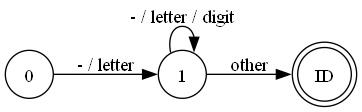
\includegraphics[
    width=0.5\textwidth]{identifier.png}
    \caption{识别标识符的\ \lstinline{DFA}}
    \label{fig:识别标识符的DFA}
\end{figure}

同时,能够被该\ \lstinline{DFA}\ 识别的字符串除了标识符以外还可能是关键字,因为所有关键字的定义也满足标识符的定义。所以还应在\ \lstinline{KeyWord}\ 表中查找被识别出来的字符串,看能否查找到。若能,则说明识别到的字符串是关键字;若不能,则说明识别到的字符串是标识符,同时将字符串加入到\ \lstinline{id_table}\ 中,以便通过下标索引值能够在\ \lstinline{id_table}\ 中找到标识符所对应的属性值。

\subsubsection{常数的识别}
~\\
\textbf{常数可以按照两类标准分类:}
\begin{itemize}
    \item 以\ 0\ 开头还是非\ 0\ 数字开头还是\ .\ 开头
    \item 整型常数还是浮点型常数
\end{itemize}
~\\
\textbf{其中以\ 0\ 开头的常数又可以分为:}
\begin{itemize}
    \item 整数\ 0
    \item 以\ 0\ 开头的八进制整型常数
    \item 以\ 0\ 开头的十六进制整型常数
    \item 以\ 0\ 开头的浮点型常数
\end{itemize}
~\\
\textbf{其中以非\ 0\ 数字开头的常数又可以分为:}
\begin{itemize}
    \item 十进制整型常数
    \item 浮点型常数
\end{itemize}
~\\
\textbf{其中以\ .\ 开头的常数只能为浮点型常数}

~\\
\textbf{其中整形常数又可以分为:}
\begin{itemize}
    \item 十进制整型常数
    \item 八进制整型常数
    \item 十六进制整型常数
\end{itemize}
~\\
\textbf{其中浮点型常数又可以分为:}
\begin{itemize}
    \item\ \lstinline{float (f / F 后缀)}
    \item\ \lstinline{double (无后缀)}
    \item\ \lstinline{long double (l / L 后缀)}
\end{itemize}
~\\
\textbf{各种进制的整型常数又可以分为:}
\begin{itemize}
    \item\ \lstinline{int (无后缀)}
    \item\ \lstinline{unsigned int (u / U 后缀)}
    \item\ \lstinline{long (l / L 后缀)}
    \item\ \lstinline{unsigned long ((u / U) + (l / L) 后缀)}
    \item\ \lstinline{long long ((l / L) + (l / L) 后缀)}
    \item\ \lstinline{unsigned long long((u / U) + (l / L) + (l / L) 后缀)}
\end{itemize}
~\\

根据以上分类,采用\ \lstinline{dot}\ 语言对识别常数的\ \lstinline{DFA} 进行定义:
\begin{lstlisting}
digraph G{
    rankdir = LR
    splines = ortho
    node[shape = circle]
    DOT[shape = doublecircle, label = "DOT(4)"]
    INT[shape = doublecircle]
    UINT[shape = doublecircle, label = "UINT(30)"]
    ULONG[shape = doublecircle, label = "ULONG(32)"]
    ULONGLONG[shape = doublecircle]
    LONG[shape = doublecircle, label = "LONG(31)"]
    LONGLONG[shape = doublecircle]
    FLOAT[shape = doublecircle]
    DOUBLE[shape = doublecircle]
    LONGDOUBLE[shape = doublecircle]
    0 -> 2 [label = "digit(except 0)"]
    0 -> 3 [label = "0"]
    0 -> DOT [label = "."]
    2 -> 2 [label = "digit"]
    2 -> 22 [label = "."]
    2 -> 23 [label = "e / E"]
    2 -> UINT [label = "u / U"]
    2 -> LONG [label = "l / L"]
    UINT -> ULONG [label = "l / L"]
    ULONG -> ULONGLONG [label = "l / L"]
    LONG -> LONGLONG [label = "l / L"]
    2 -> INT [label = "INT"]
    22 -> 22 [label = "digit"]
    22 -> 23 [label = "e / E"]
    22 -> FLOAT [label = "f / F"]
    22 -> LONGDOUBLE [label = "l / L"]
    22 -> DOUBLE [label = "other"]
    23 -> 24 [label = "+ / -"]
    23 -> 25 [label = "digit"]
    24 -> 25 [label = "digit"]
    25 -> 25 [label = "digit"]
    25 -> FLOAT [label = "f / F"]
    25 -> LONGDOUBLE [label = "l / L"]
    25 -> DOUBLE [label = "other"]
    3 -> 22 [label = "."]
    3 -> 26 [label = "oct_digt"]
    3 -> 27 [label = "8 / 9"]
    3 -> 23 [label = "e / E"]
    3 -> 28 [label = "x / X"]
    3 -> INT [label = "other"]
    3 -> UINT [label = "u / U"]
    3 -> LONG [label = "l / L"]
    26 -> 27 [label = "8 / 9"]
    26 -> 26 [label = "oct_digit"]
    26 -> 23 [label = "e / E"]
    26 -> UINT [label = "u / U"]
    26 -> LONG [label = "l / L"]
    26 -> 22 [label = "."]
    27 -> 27 [label = "digit"]
    27 -> 22 [label = "."]
    27 -> 23 [label = "e / E"]
    28 -> 29 [label = "hex_digit"]
    29 -> 29 [label = "hex_digit"]
    29 -> INT [label = "other"]
    29 -> UINT [label = "u / U"]
    29 -> LONG [label = "l / L"]
    DOT -> 22 [label = "digit"]
}
\end{lstlisting}

编译得到识别常数的\ \lstinline{DFA}\ 的状态转移图:\ \textbf{图\ \ref{fig:识别常数的DFA}}

\begin{figure}[!htb]
    \centering
    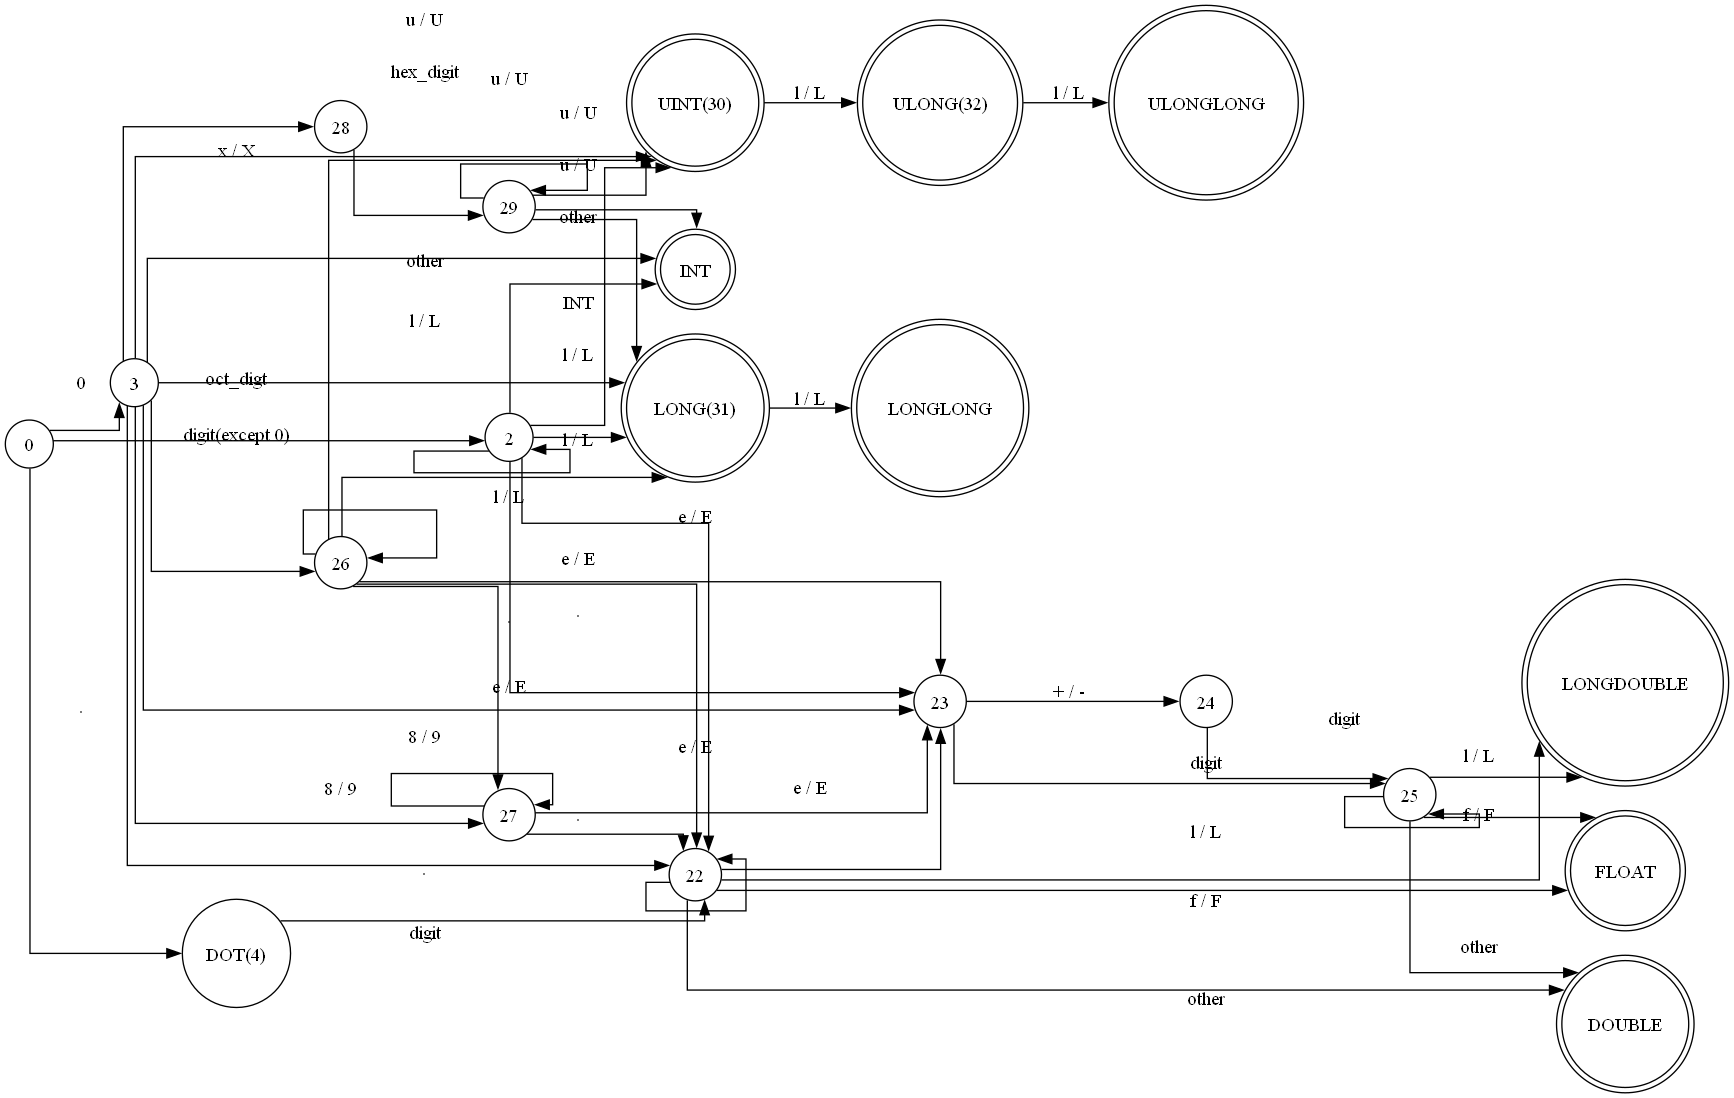
\includegraphics[
    width= 1 \textwidth]{digit.png}
    \caption{识别常数的\ \lstinline{DFA}}
    \label{fig:识别常数的DFA}
\end{figure}

识别出的常数分为九类:\ \lstinline{INT, UINT, LONG, ULONG, LONGLONG, ULONGLONG, FLOAT, DOUBLE, LONGDOUBLE},这九类是按照常数是整型还是浮点型以及常数的后缀类型来划分的。

\subsubsection{字符常量的识别}

处理字符常量的一个关键点在于能够准确识别转义字符,所以当在\ \lstinline{''}\ 中识别到\ \textbackslash\ 时要做特殊的判断,同时还要对识别到的转义字符的合法性进行判断,eg.\lstinline{'\p'}\ 便是一个非法的转义字符,设计的词法分析程序应当能判别转义字符的合法性,并在非法时输出相应错误提示便于编程人员对源程序进行修改。

下面给出用\ \lstinline{DOT}\ 语言定义的识别字符常量的\ \lstinline{DFA}:

\begin{lstlisting}
digraph G{
    rankdir=LR
    splines = line
    node[shape = circle]
    CHAR [shape = doublecircle, fontsize = 10]
    ERROR [shape = doublecircle, label = "ERROR(21)", fontsize = 10]
    0 -> 7 [label = "'"]
    7 -> ERROR [label = "' / \\n / EOF "]
    7 -> 35 [label = "other"]
    7 -> 34 [label = "\\"]
    34 -> 35 [label = "legal escape characters"]
    35 -> CHAR [label = "'"]
}
\end{lstlisting}

编译得到\ \lstinline{png}\ 格式的状态转移图:\textbf{图\ \ref{fig:识别字符常量的DFA}}

\begin{figure}[!htb]
    \centering
    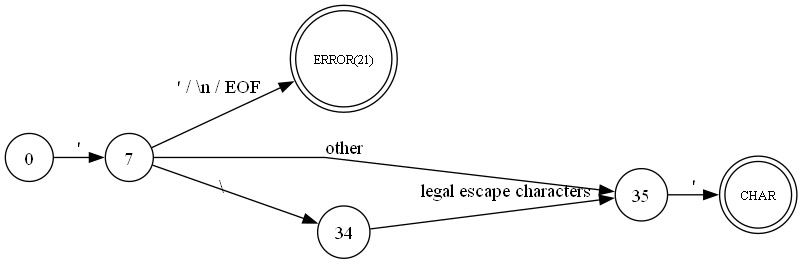
\includegraphics[
    width= 0.75 \textwidth]{char.png}
    \caption{识别字符常量的\ \lstinline{DFA}}
    \label{fig:识别字符常量的DFA}
\end{figure}

除了转义字符非法的错误外,我们还需要考虑字符常量为空,eg.\lstinline{''},以及字符常量未闭合的错误情况,eg.\lstinline{'a}。

\subsubsection{字符串常量的识别}

字符串常量的识别与字符常量的识别类似,同样需要对转义字符进行检测并判断其合法性,同时需要考虑未闭合的错误情况,但字符串常量允许为空。

下面给出用\ \lstinline{DOT}\ 语言定义的识别字符串常量的\ \lstinline{DFA}:

\begin{lstlisting}
digraph G{
    rankdir=LR
    splines = line
    node[shape = circle]
    STRING [shape = doublecircle, fontsize = 10]
    ERROR [shape = doublecircle, label = "ERROR(21)", fontsize = 10]
    0 -> 6 [label = "\""]
    6 -> 6 [label = "other"]
    6 -> ERROR [label = "\\n / EOF"]
    6 -> 33 [label = "\\"]
    6 -> STRING [label = "\""]
    33 -> 6 [label = "legal escape characters"]
}
\end{lstlisting}

编译得到\ \lstinline{png}\ 格式的状态转移图:\textbf{图\ \ref{fig:识别字符串常量的DFA}}

\begin{figure}[!htb]
    \centering
    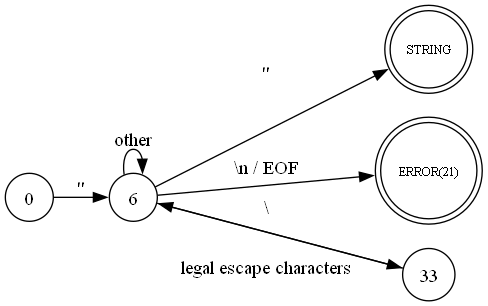
\includegraphics[
    width= 0.55 \textwidth]{string.png}
    \caption{识别字符串常量的\ \lstinline{DFA}}
    \label{fig:识别字符串常量的DFA}
\end{figure}

\subsubsection{运算符的识别}

运算符的种类较多,但识别方法类似,下面给出比较典型的\ \lstinline{'<'}\ 符号簇的识别过程。

当识别到\ \lstinline{'<'}\ 符号时我们无法第一时间判断其符号类型,因为它既可能是\ \lstinline{<}\ 也可能是\ \lstinline{<=, <<, <<=}\ 等符号的前缀,因此需要\textbf{超前扫描}。

下面给出用\ \lstinline{DOT}\ 语言定义的识别\ \lstinline{'<'}\ 符号簇\ 的\lstinline{DFA}:

\begin{lstlisting}
digraph G{
    rankdir=LR
    node[shape = circle]
    RELATION_OPERATOR [shape = doublecircle, fontsize = 10]
    ASSIGN_OPERATOR [shape = doublecircle, fontsize = 10]
    BITWISE_OPERATOR [shape = doublecircle, fontsize = 10]
    0 -> 16 [label = "<"]
    16 -> 39 [label = "<"]
    16 -> RELATION_OPERATOR [label = "= / other"]
    39 -> ASSIGN_OPERATOR [label = "="]
    39 -> BITWISE_OPERATOR [label = "other"]
}
\end{lstlisting}

编译得到\ \lstinline{png}\ 格式的状态转移图:\textbf{图\ \ref{fig:识别 '<' 符号簇的DFA}}

\begin{figure}[!htb]
    \centering
    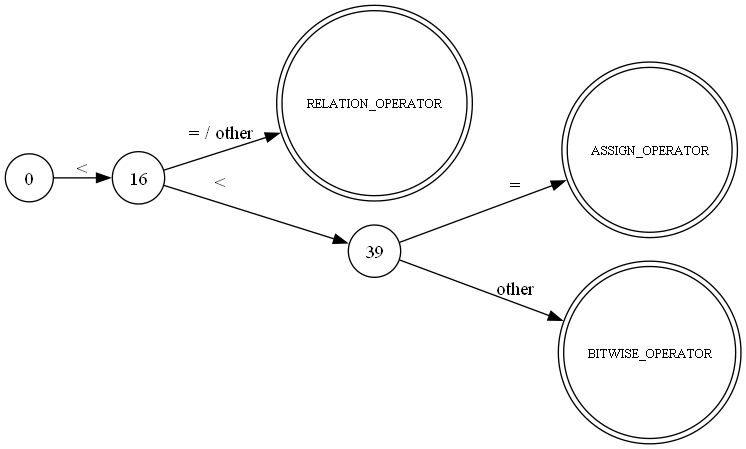
\includegraphics[
    width= 0.75 \textwidth]{less_than.png}
    \caption{识别\ \lstinline{'<'}\ 符号簇的\ \lstinline{DFA}}
    \label{fig:识别 '<' 符号簇的DFA}
\end{figure}

最终识别到符号可能为属于\ \lstinline{RELATION_OPERATOR}\ 的\ \lstinline{<}\ 或\ \lstinline{<=},或者属于\ \lstinline{ASSIGN_OPERATOR}\ 的\ \lstinline{<<=},亦或者属于\ \lstinline{BITWISE_OPERATOR}\ 的\ \lstinline{<<}。

\subsubsection{注释的识别}

注释分为单行注释和多行注释,二者都以\ \lstinline{/}\ 开头。单行注释遇到\ \lstinline{\n}\ 或\ \lstinline{EOF}\ 结束;多行注释当匹配到对应的\ \lstinline{*/}\ 时结束,因此需要进行闭合检测,若读到文件末尾还没有与\ \lstinline{/*}\ 匹配的\ \lstinline{*/},就输出多行注释未闭合的错误。

下面给出用\ \lstinline{DOT}\ 语言定义的识别注释的\ \lstinline{DFA}:

\begin{lstlisting}
digraph G{
    rankdir=LR
    node[shape = circle]
    ANNOTATION [shape = doublecircle, fontsize = 10]
    0 -> 11 [label = "/"]
    11 -> 36 [label = "/"]
    11 -> 37 [label = "*"]
    36 -> 36 [label = "other"]
    36 -> ANNOTATION [label = "\\n / EOF"]
    37 -> 37 [label = "other"]
    37 -> 38 [label = "*"]
    38 -> 37 [label = "other"]
    38 -> 38 [label = "*"]
    38 -> ANNOTATION [label = "/"]
}
\end{lstlisting}

编译得到\ \lstinline{png}\ 格式的状态转移图:\textbf{图\ \ref{fig:识别注释的DFA}}

\begin{figure}[!htb]
    \centering
    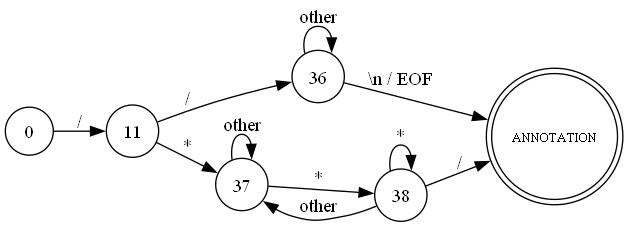
\includegraphics[
    width= 0.75 \textwidth]{annotation.png}
    \caption{识别注释\ \lstinline{DFA}}
    \label{fig:识别注释的DFA}
\end{figure}


\subsubsection{其他记号的识别}

其他记号识别的分析过程与上面类似,由于篇幅限制,此处不再过多赘述。

\subsection{词法错误}

\subsubsection{错误类型的定义}

\begin{lstlisting}
enum ErrorType
{
    UNKNOWN_SYMBOL,     // 未知符号
    ILLEGAL_NUMBERS,    // 非法数字
    UNCLOSED_STRING,    // 未闭合字符串
    UNCLOSED_CHAR,      // 未闭合字符
    EMPTY_CHAR,         // 空字符
    ILLEGAL_ESCAPE,     // 非法转义字符
    UNCLOSED_ANNOTATION // 未闭合注释
};
\end{lstlisting}

\subsubsection{错误的处理}

当遇到词法错误时,词法分析函数会跳转到状态\ \lstinline{21}\ 处理错误。

错误处理的\ \lstinline{DFA}\ 的定义:
\begin{lstlisting}
digraph G{
    rankdir=LR
    node[shape = circle]
    ERROR [shape = doublecircle, label = "ERROR(21)", fontsize = 10]
    ERROR -> ERROR [label = "other"]
    ERROR -> 0 [label = "',' / ' ' / '\\t' / '\\n' / ';' / EOF"]
}
\end{lstlisting}

编译得到\ \lstinline{png}\ 格式的状态转移图:\textbf{图\ \ref{fig:错误处理的的DFA}}

\begin{figure}[!htb]
    \centering
    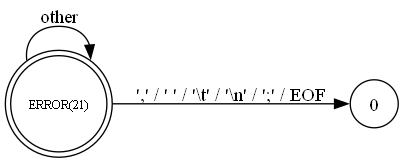
\includegraphics[
    width= 0.5 \textwidth]{error.png}
    \caption{错误处理的\ \lstinline{DFA}}
    \label{fig:错误处理的的DFA}
\end{figure}

将错误处理的\ \lstinline{DFA}\ 用\ \lstinline{C++}\ 代码实现:
\begin{lstlisting}
case 21:
    if (c == ' ' || c == '\t' || c == '\n' || c == EOF || c == ',' || c == ';')
    {
        go_back(fin, char_num, col);
        error(error_type, line, col, buffer);
        state = 0;
    }
    else
    {
        next_char(fin, char_num, c, buffer, col);
        state = 21;
    }
    break;
\end{lstlisting}

错误处理的准则:继续读入字符,并将字符加入存储错误记号的\ \lstinline{buffer}\ 中,直到读到\ \lstinline{' ' or '\t' or '\n' or EOF or ',' or ';'}\ 时停止,并回退一个字符,再调用错误输出函数\ \lstinline{error}。

错误输出函数\ \lstinline{error}\ 按照\ \lstinline{"Error: line:col: 错误类型: 错误内容"}\ 的格式输出错误信息。

eg.\ \lstinline{Error: 29:14:Illegal const numbers: 09}

处理完错误后,词法分析函数继续执行,对剩余的文件流进行词法分析,实现了对源程序中出现的错误进行适当的恢复,使词法分析可以继续进行的功能。

\subsection{记号流的存储及输出}

识别出的记号通过定义在\ \lstinline{lexical_analysis.h}\ 中的\ \lstinline{add_token}\ 函数加入到记号流\ \lstinline{vector<Token> &token_streams}\ 中。

\begin{lstlisting}
/**
 * @brief 向记号流添加记号
 *
 * @param buffer 当前读入的记号
 * @param token_streams 记号流
 * @param type 记号类型
 * @param id_table 标识符表
 * @param str_table 字符串表
 * @param line 当前行数
 * @param col 当前列数
 * @param base 记号的基数
 */
void add_token(string buffer, vector<Token> &token_streams, const TokenType type, vector<string> &id_table, vector<string> &str_table, const int line, const int col, const int base);
\end{lstlisting}

记号流通过定义在\ \lstinline{output.h}\ 中的\ \lstinline{output}\ 函数以特定格式输出,详细格式见\textbf{程序测试}中的\textbf{测试结果}。

\begin{lstlisting}
/**
 * @brief 输出记号流
 * 
 * @param token_streams 记号流  
 * @param id_table 标识符表
 * @param str_table 字符串表
 * @param char_num 字符总数
 * @param line 行数
 */
void output(const vector<Token> &token_streams, const vector<string> &id_table, const vector<string> &str_table, const int char_num, const int line);

\end{lstlisting}

\section{程序测试}

\subsection{测试集\ 1}

此测试集用于测试程序是否能够准确识别标识符及关键字。

\subsubsection{测试内容}

\begin{lstlisting}
#include <stdio.h>

int main()
{
    int _123;
    unsigned int _abc;
    long abc_;
    long long abc_123;
    unsigned long long 123abc;
    double _double;
    char 345;
}
\end{lstlisting}

\subsubsection{测试结果}

\begin{lstlisting}
========================Token Streams========================
<3:1><Keyword, int>     <3:5><Identifier, main>
<3:9><Left Parenthese, (>       <3:10><Right Parenthese, )>
<4:1><Left Brace, {>    <5:5><Keyword, int>
<5:9><Identifier, _123> <5:13><Semicolon, ;>
<6:5><Keyword, unsigned>        <6:14><Keyword, int>
<6:18><Identifier, _abc>        <6:22><Semicolon, ;>
<7:5><Keyword, long>    <7:10><Identifier, abc_>
<7:14><Semicolon, ;>    <8:5><Keyword, long>
<8:10><Keyword, long>   <8:15><Identifier, abc_123>
<8:22><Semicolon, ;>    <9:5><Keyword, unsigned>
<9:14><Keyword, long>   <9:19><Keyword, long>
<9:24><Int, 123>        <9:27><Identifier, abc>
<9:30><Semicolon, ;>    <10:5><Keyword, double>
<10:12><Identifier, _double>    <10:19><Semicolon, ;>
<11:5><Keyword, char>   <11:10><Int, 345>
<11:13><Semicolon, ;>   <12:1><Right Brace, }>

========Analysis Result========
Total lines: 12
Total characters: 155
Total tokens: 32
Total keywords: 12
Total identifiers: 7
Total const strings: 0
Total const characters: 0
Total const integers: 2
Total const floats: 0
Total operators: 0
Total others: 11
\end{lstlisting}

\subsubsection{结果分析}

对于两个非法标识符\ \lstinline{123abc}\ 和\ \lstinline{345},词法分析程序对前者的识别结果为\ \lstinline{<9:24><Int, 123>}\ 和\ \lstinline{<9:27><Identifier, abc>}, 符合预期设想;对后者的识别结果为\ \lstinline{<11:10><Int, 345>},也符合预期设想。标识符虽然非法,但词法分析程序未输出错误信息,因为对于该类错误的判定属于语法分析的任务。

其余合法的标识符和关键字也都能够被准确识别。对于记号类别的统计信息也符合预期。

\subsection{测试集\ 2}

此测试集用于测试程序是否能够准确识别字符常量并判定其合法性。

\subsubsection{测试内容}

\begin{lstlisting}
#include <stdio.h>

int main()
{
    'a';
    '\0', '\a', '\b', '\t', '\n', '\v', '\f', '\r', '\"', '\'', '\?', '\\';
    '';
    'b;
    '\p';
}
\end{lstlisting}

\subsubsection{测试结果}

\begin{lstlisting}
Error: 7:5:Empty const char: ''
Error: 8:5:Unclosed const char: 'b
Error: 9:5:Illegal escape character: '\p'

========================Token Streams========================
<3:1><Keyword, int>     <3:5><Identifier, main>
<3:9><Left Parenthese, (>       <3:10><Right Parenthese, )>
<4:1><Left Brace, {>    <5:7><Char, a>
<5:8><Semicolon, ;>     <6:7><Char, >
<6:9><Comma, ,> <6:13><Char, >
<6:15><Comma, ,>        <6:19><Char,>
<6:21><Comma, ,>        <6:25><Char,    >
<6:27><Comma, ,>        <6:31><Char, 
>
<6:33><Comma, ,>        <6:37><Char, 
>
<6:39><Comma, ,>        <6:43><Char, 
>
>6:45><Comma, ,>        <6:49><Char, 
<6:51><Comma, ,>        <6:55><Char, ">
<6:57><Comma, ,>        <6:61><Char, '>
<6:63><Comma, ,>        <6:67><Char, ?>
<6:69><Comma, ,>        <6:73><Char, \>
<6:75><Semicolon, ;>    <7:7><Semicolon, ;>
<8:7><Semicolon, ;>     <9:9><Semicolon, ;>
<10:1><Right Brace, }>

========Analysis Result========
Total lines: 10
Total characters: 126
Total tokens: 35
Total keywords: 1
Total identifiers: 1
Total const strings: 0
Total const characters: 13
Total const integers: 0
Total const floats: 0
Total operators: 0
Total others: 20
\end{lstlisting}

\subsubsection{结果分析}

对于三个非法的字符常量\ \lstinline{‘’},\lstinline{‘b},\lstinline{'\p'},词法分析程序都能识别出错误,并输出相应错误信息(测试结果\ 1-3\ 行),符合预期设想。

其余合法的字符常量也都能够被准确识别。对于记号类别的统计信息也符合预期。

注:由于记号属性值存储的是记号的真实值,例如换行符的输出就是一个真实的换行,但由此也导致有些转义字符的输出无法显示。

\subsection{测试集\ 3}

此测试集用于测试程序是否能够准确识别字符串常量并判定其合法性。

\subsubsection{测试内容}

\begin{lstlisting}
#include <stdio.h>

int main()
{
    "";
    "abc";
    "def;
    "abc\"";
    "def\p";
}
\end{lstlisting}

\subsubsection{测试结果}

\begin{lstlisting}
Error: 7:5:Unclosed const string: "def;
Error: 9:5:Illegal escape character: "def\p"

========================Token Streams========================
<3:1><Keyword, int>     <3:5><Identifier, main>
<3:9><Left Parenthese, (>       <3:10><Right Parenthese, )>
<4:1><Left Brace, {>    <5:7><String, >
<5:7><Semicolon, ;>     <6:7><String, abc>
<6:10><Semicolon, ;>    <8:7><String, abc\">
<8:12><Semicolon, ;>    <9:12><Semicolon, ;>
<10:1><Right Brace, }>

========Analysis Result========
Total lines: 10
Total characters: 70
Total tokens: 13
Total keywords: 1
Total identifiers: 1
Total const strings: 3
Total const characters: 0
Total const integers: 0
Total const floats: 0
Total operators: 0
Total others: 8
\end{lstlisting}

\subsubsection{结果分析}

对于两个非法的字符串常量\ \lstinline{"def}\ 和\ \lstinline{"def\p"},词法分析程序都能识别出错误,并输出相应错误信息(测试结果\ 1-2\ 行),符合预期设想。

其余合法的字符串常量也都能够被准确识别。对于记号类别的统计信息也符合预期。

\subsection{测试集\ 4}

此测试集用于测试程序是否能够准确识别常数并判定其合法性。

\subsubsection{测试内容}

\begin{lstlisting}
#include <stdio.h>

int main()
{
    123, 123u, 123l, 123ul, 123ll, 123ull;
    123., 123.456, 123.456e5, 123.456e+5, 123.456e-5, 123e5, 123.e5;
    123.456e+5f, 123.456e+5l;
    0, 0U, 0L, 0UL, 0LL, 0ULL;
    0123, 0234U, 0345L, 0456UL, 0567LL;
    0789.;
    0789;
    0x123, 0x234U, 0x345L, 0x456uL, 0x789lL, 0x89aULl, 0x9ab,0xabc;
    0.123, 0.123e5, 0.123e+5, 0.123e-5;
    123e+a;
    123e-;
    .123F, .123e5L, .123e+5, .123e-5;
}
\end{lstlisting}

\subsubsection{测试结果}

\begin{lstlisting}
Error: 11:5:Illegal const numbers: 0789
Error: 14:5:Illegal const numbers: 123e+a
Error: 15:5:Illegal const numbers: 123e-

========================Token Streams========================
<3:1><Keyword, int>     <3:5><Identifier, main>
<3:9><Left Parenthese, (>       <3:10><Right Parenthese, )>
<4:1><Left Brace, {>    <5:5><Int, 123>
<5:8><Comma, ,> <5:10><Unsigned Int, 123>
<5:13><Comma, ,>        <5:15><Long, 123>
<5:18><Comma, ,>        <5:20><Unsigned Long, 123>
<5:23><Comma, ,>        <5:26><Long Long, 123>
<5:29><Comma, ,>        <5:32><Unsigned Long Long, 123>
<5:35><Semicolon, ;>    <6:5><Double, 123>
<6:9><Comma, ,> <6:11><Double, 123.456>
<6:18><Comma, ,>        <6:20><Double, 1.23456e+07>
<6:29><Comma, ,>        <6:31><Double, 1.23456e+07>
<6:41><Comma, ,>        <6:43><Double, 0.00123456>
<6:53><Comma, ,>        <6:55><Double, 1.23e+07>
<6:60><Comma, ,>        <6:62><Double, 1.23e+07>
<6:68><Semicolon, ;>    <7:6><Float, 1.23456e+07>
<7:16><Comma, ,>        <7:19><Long Double, 1.23456e+07>
<7:29><Semicolon, ;>    <8:5><Int, 0>
<8:6><Comma, ,> <8:8><Unsigned Int, 0>
<8:9><Comma, ,> <8:11><Long, 0>
<8:12><Comma, ,>        <8:14><Unsigned Long, 0>
<8:15><Comma, ,>        <8:18><Long Long, 0>
<8:19><Comma, ,>        <8:22><Unsigned Long Long, 0>
<8:23><Semicolon, ;>    <9:5><Int, 83>
<9:9><Comma, ,> <9:11><Unsigned Int, 156>
<9:15><Comma, ,>        <9:17><Long, 229>
<9:21><Comma, ,>        <9:23><Unsigned Long, 302>
<9:27><Comma, ,>        <9:30><Long Long, 375>
<9:34><Semicolon, ;>    <10:5><Double, 789>
<10:10><Semicolon, ;>   <11:9><Semicolon, ;>
<12:5><Int, 291>        <12:10><Comma, ,>
<12:12><Unsigned Int, 564>      <12:17><Comma, ,>
<12:19><Long, 837>      <12:24><Comma, ,>
<12:26><Unsigned Long, 1110>    <12:31><Comma, ,>
<12:34><Long Long, 1929>        <12:39><Comma, ,>
<12:42><Unsigned Long Long, 2202>       <12:47><Comma, ,>
<12:49><Int, 2475>      <12:54><Comma, ,>
<12:55><Int, 2748>      <12:60><Semicolon, ;>
<13:5><Double, 0.123>   <13:10><Comma, ,>
<13:12><Double, 12300>  <13:19><Comma, ,>
<13:21><Double, 12300>  <13:29><Comma, ,>
<13:31><Double, 1.23e-06>       <13:39><Semicolon, ;>
<14:11><Semicolon, ;>   <15:10><Semicolon, ;>
<16:6><Float, 0.123>    <16:10><Comma, ,>
<16:13><Long Double, 12300>     <16:19><Comma, ,>
<16:21><Double, 12300>  <16:28><Comma, ,>
<16:30><Double, 1.23e-06>       <16:37><Semicolon, ;>
<17:1><Right Brace, }>

========Analysis Result========
Total lines: 17
Total characters: 418
Total tokens: 95
Total keywords: 1
Total identifiers: 1
Total const strings: 0
Total const characters: 0
Total const integers: 25
Total const floats: 18
Total operators: 0
Total others: 50
\end{lstlisting}

\subsubsection{结果分析}

对于三个非法的常数\ \lstinline{0789},\lstinline{123e+a},\lstinline{123e-},词法分析程序都能识别出错误,并输出相应错误信息(测试结果\ 1-3\ 行),符合预期设想。

注:\lstinline{0789}\ 非法是因为以\ \lstinline{0}\ 开头的常数若是十进制则必须是浮点数,所以\ \lstinline{0789.}\ 是合法的。

其余合法的常数也都能够被准确识别,同时程序也能够根据常数的后缀判断常数的具体类型。对于十进制、八进制、十六进制的常数程序也能够准确辨别,并在输出属性值时进行进制转换,以十进制格式输出,例如对于\ \lstinline{0123}\ 的识别为\ \lstinline{<9:5><Int , 83>}\ 。对于记号类别的统计信息也符合预期。

\subsection{测试集\ 5}

此测试集用于测试程序是否能够准确识别运算符、其他符号以及注释。

\subsubsection{测试内容}

\begin{lstlisting}
#include <stdio.h>

int main()
{
    +, -, *, /, %, ++, --, &&, ||, !, &, |, ~, ^, << ;
    >>, =, +=, -=, *=, /=, %=, &=, |=, ^=, <<=, >>=, == ;
    !=, >, <, >=, <= ;

    ?, :, ;
    , [, ], (, ),
    { , }, ., , , ->;

    // this is a sigle line annotation

    /* this is a multiple line annotation


    */

    ` // UNKNOWN_SYMBOL
}

/* this is an unclosed multiple line annotation

\end{lstlisting}

\subsubsection{测试结果}

\begin{lstlisting}
Error: 20:5:Unknown symbol: `
Error: 24:1:/* this is an unclosed multiple line annotation


========================Token Streams========================
<3:1><Keyword, int>     <3:5><Identifier, main>
<3:9><Left Parenthese, (>       <3:10><Right Parenthese, )>
<4:1><Left Brace, {>    <5:5><Agorithm Operator, +>
<5:6><Comma, ,> <5:8><Agorithm Operator, ->
<5:9><Comma, ,> <5:11><Agorithm Operator, *>
<5:12><Comma, ,>        <5:14><Agorithm Operator, />
<5:15><Comma, ,>        <5:17><Agorithm Operator, %>
<5:18><Comma, ,>        <5:20><Agorithm Operator, ++>
<5:22><Comma, ,>        <5:24><Agorithm Operator, -->
<5:26><Comma, ,>        <5:28><Logical Operator, &&>
<5:30><Comma, ,>        <5:32><Logical Operator, ||>
<5:34><Comma, ,>        <5:36><Logical Operator, !>
<5:37><Comma, ,>        <5:39><Bitwise Operator, &>
<5:40><Comma, ,>        <5:42><Bitwise Operator, |>
<5:43><Comma, ,>        <5:45><Bitwise Operator, ~>
<5:46><Comma, ,>        <5:48><Bitwise Operator, ^>
<5:49><Comma, ,>        <5:51><Bitwise Operator, <<>
<5:54><Semicolon, ;>    <6:5><Bitwise Operator, >>>
<6:7><Comma, ,> <6:9><Assign Operator, =>
<6:10><Comma, ,>        <6:12><Assign Operator, +=>
<6:14><Comma, ,>        <6:16><Assign Operator, -=>
<6:18><Comma, ,>        <6:20><Assign Operator, *=>
<6:22><Comma, ,>        <6:24><Assign Operator, /=>
<6:26><Comma, ,>        <6:28><Assign Operator, %=>
<6:30><Comma, ,>        <6:32><Assign Operator, &=>
<6:34><Comma, ,>        <6:36><Assign Operator, |=>
<6:38><Comma, ,>        <6:40><Assign Operator, ^=>
<6:42><Comma, ,>        <6:44><Assign Operator, <<=>
<6:47><Comma, ,>        <6:49><Assign Operator, >>=>
<6:52><Comma, ,>        <6:54><Relation Operator, ==>
<6:57><Semicolon, ;>    <7:5><Relation Operator, !=>
<7:7><Comma, ,> <7:9><Relation Operator, >>
<7:10><Comma, ,>        <7:12><Relation Operator, <>
<7:13><Comma, ,>        <7:15><Relation Operator, >=>
<7:17><Comma, ,>        <7:19><Relation Operator, <=>
<7:22><Semicolon, ;>    <9:5><Question Mark, ?>
<9:6><Comma, ,> <9:8><Colon, :>
<9:9><Comma, ,> <9:11><Semicolon, ;>
<10:5><Comma, ,>        <10:7><Left Square Bracket, [>
<10:8><Comma, ,>        <10:10><Right Square Bracket, ]>
<10:11><Comma, ,>       <10:13><Left Parenthese, (>
<10:14><Comma, ,>       <10:16><Right Parenthese, )>
<10:17><Comma, ,>       <11:5><Left Brace, {>
<11:7><Comma, ,>        <11:9><Right Brace, }>
<11:10><Comma, ,>       <11:12><Dot, .>
<11:13><Comma, ,>       <11:15><Comma, ,>
<11:17><Comma, ,>       <11:19><Arrow, ->>
<11:21><Semicolon, ;>   <21:1><Right Brace, }>

========Analysis Result========
Total lines: 24
Total characters: 371
Total tokens: 96
Total keywords: 1
Total identifiers: 1
Total const strings: 0
Total const characters: 0
Total const integers: 0
Total const floats: 0
Total operators: 33
Total others: 61
PS E:\Desktop\5th_Semester_Labs\Compilation_Principles_and_Techniques\Lab1>  & 'c:\Users\SteveZL\.vscode\extensions\ms-vscode.cpptools-1.17.5-win32-x64\debugAdapters\bin\WindowsDebugLauncher.exe' '--stdin=Microsoft-MIEngine-In-yxqtahyz.u5j' '--stdout=Microsoft-MIEngine-Out-eh5upnjn.hmj' '--stderr=Microsoft-MIEngine-Error-lxyy031h.y4q' '--pid=Microsoft-MIEngine-Pid-yxw2130l.2jh' '--dbgExe=C:\Program Files\mingw64\bin\gdb.exe' '--interpreter=mi'
test5.cpp
Error: 20:5:Unknown symbol: `
Error: 24:1:Unclosed annotation: /* this is an unclosed multiple line annotation


========================Token Streams========================
<3:1><Keyword, int>     <3:5><Identifier, main>
<3:9><Left Parenthese, (>       <3:10><Right Parenthese, )>
<4:1><Left Brace, {>    <5:5><Agorithm Operator, +>
<5:6><Comma, ,> <5:8><Agorithm Operator, ->
<5:9><Comma, ,> <5:11><Agorithm Operator, *>
<5:12><Comma, ,>        <5:14><Agorithm Operator, />
<5:15><Comma, ,>        <5:17><Agorithm Operator, %>
<5:18><Comma, ,>        <5:20><Agorithm Operator, ++>
<5:22><Comma, ,>        <5:24><Agorithm Operator, -->
<5:26><Comma, ,>        <5:28><Logical Operator, &&>
<5:30><Comma, ,>        <5:32><Logical Operator, ||>
<5:34><Comma, ,>        <5:36><Logical Operator, !>
<5:37><Comma, ,>        <5:39><Bitwise Operator, &>
<5:40><Comma, ,>        <5:42><Bitwise Operator, |>
<5:43><Comma, ,>        <5:45><Bitwise Operator, ~>
<5:46><Comma, ,>        <5:48><Bitwise Operator, ^>
<5:49><Comma, ,>        <5:51><Bitwise Operator, <<>
<5:54><Semicolon, ;>    <6:5><Bitwise Operator, >>>
<6:7><Comma, ,> <6:9><Assign Operator, =>
<6:10><Comma, ,>        <6:12><Assign Operator, +=>
<6:14><Comma, ,>        <6:16><Assign Operator, -=>
<6:18><Comma, ,>        <6:20><Assign Operator, *=>
<6:22><Comma, ,>        <6:24><Assign Operator, /=>
<6:26><Comma, ,>        <6:28><Assign Operator, %=>
<6:30><Comma, ,>        <6:32><Assign Operator, &=>
<6:34><Comma, ,>        <6:36><Assign Operator, |=>
<6:38><Comma, ,>        <6:40><Assign Operator, ^=>
<6:42><Comma, ,>        <6:44><Assign Operator, <<=>
<6:47><Comma, ,>        <6:49><Assign Operator, >>=>
<6:52><Comma, ,>        <6:54><Relation Operator, ==>
<6:57><Semicolon, ;>    <7:5><Relation Operator, !=>
<7:7><Comma, ,> <7:9><Relation Operator, >>
<7:10><Comma, ,>        <7:12><Relation Operator, <>
<7:13><Comma, ,>        <7:15><Relation Operator, >=>
<7:17><Comma, ,>        <7:19><Relation Operator, <=>
<7:22><Semicolon, ;>    <9:5><Question Mark, ?>
<9:6><Comma, ,> <9:8><Colon, :>
<9:9><Comma, ,> <9:11><Semicolon, ;>
<10:5><Comma, ,>        <10:7><Left Square Bracket, [>
<10:8><Comma, ,>        <10:10><Right Square Bracket, ]>
<10:11><Comma, ,>       <10:13><Left Parenthese, (>
<10:14><Comma, ,>       <10:16><Right Parenthese, )>
<10:17><Comma, ,>       <11:5><Left Brace, {>
<11:7><Comma, ,>        <11:9><Right Brace, }>
<11:10><Comma, ,>       <11:12><Dot, .>
<11:13><Comma, ,>       <11:15><Comma, ,>
<11:17><Comma, ,>       <11:19><Arrow, ->>
<11:21><Semicolon, ;>   <21:1><Right Brace, }>

========Analysis Result========
Total lines: 24
Total characters: 371
Total tokens: 96
Total keywords: 1
Total identifiers: 1
Total const strings: 0
Total const characters: 0
Total const integers: 0
Total const floats: 0
Total operators: 33
Total others: 61
\end{lstlisting}

\subsubsection{结果分析}

对于未知字符错误:\lstinline{`}\ 和未闭合的多行注释错误:\lstinline{/* this is an unclosed multiple line annotation},词法分析程序都能够准确识别,并输出相应错误信息(测试结果\ 1-2\ 行),符合预期设想。

对运算符的识别实现了\textbf{超前扫描}功能,能够区分例如\ \lstinline{<, <=, <<, <<=}\ 等前缀相同的运算符。同时对于\ \lstinline{., ;, [}\ 等其他符号也能够准确识别。遇到注释能够识别并跳过。对于记号类别的统计信息也符合预期。

\subsection{测试集\ 6}

此测试集用于综合测试程序。

\subsubsection{测试内容}

\begin{lstlisting}
#include <stdio.h>
#include <math.h>

struct node
{
    int a;
    int b;
};

int main()
{
    int i = 123;
    unsigned int ui = 0456u;
    long long ll = 0x123456789abcdefll;

    // this is a single line comment

    float f = 1.f;
    double d = 1.234e+10;
    long double ld = 1.234e-10l;

    struct node n1;
    struct node *temp = &n1;
    temp->b = 123ull;

    /*
    this is a multi-line comment
    */

    char c = '\?';
    if (c <= '\f' && fabs(d - 123e7) > 1e-10)
    {
        c = '\f';
        i++;
        ui << 1;
        ll <<= 2;
        f = (i == 123) ? 1.0 : 0;
        ld -= 1.0;
        n1.a = 123;
    }
    printf("This is a string");
    
    return 0;
}
\end{lstlisting}

\subsubsection{测试结果}

\begin{lstlisting}
========================Token Streams========================
<4:1><Keyword, struct>  <4:8><Identifier, node>
<5:1><Left Brace, {>    <6:5><Keyword, int>
<6:9><Identifier, a>    <6:10><Semicolon, ;>
<7:5><Keyword, int>     <7:9><Identifier, b>
<7:10><Semicolon, ;>    <8:1><Right Brace, }>
<8:2><Semicolon, ;>     <10:1><Keyword, int>
<10:5><Identifier, main>        <10:9><Left Parenthese, (>
<10:10><Right Parenthese, )>    <11:1><Left Brace, {>
<12:5><Keyword, int>    <12:9><Identifier, i>
<12:11><Assign Operator, =>     <12:13><Int, 123>
<12:16><Semicolon, ;>   <13:5><Keyword, unsigned>
<13:14><Keyword, int>   <13:18><Identifier, ui>
<13:21><Assign Operator, =>     <13:23><Unsigned Int, 302>
<13:27><Semicolon, ;>   <14:5><Keyword, long>
<14:10><Keyword, long>  <14:15><Identifier, ll>
<14:18><Assign Operator, =>     <14:21><Long Long, 81985529216486895>
<14:38><Semicolon, ;>   <18:5><Keyword, float>
<18:11><Identifier, f>  <18:13><Assign Operator, =>
<18:16><Float, 1>       <18:18><Semicolon, ;>
<19:5><Keyword, double> <19:12><Identifier, d>
<19:14><Assign Operator, =>     <19:16><Double, 1.234e+10>
<19:25><Semicolon, ;>   <20:5><Keyword, long>
<20:10><Keyword, double>        <20:17><Identifier, ld>
<20:20><Assign Operator, =>     <20:23><Long Double, 1.234e-10>
<20:32><Semicolon, ;>   <22:5><Keyword, struct>
<22:12><Identifier, node>       <22:17><Identifier, n1>
<22:19><Semicolon, ;>   <23:5><Keyword, struct>
<23:12><Identifier, node>       <23:17><Agorithm Operator, *>
<23:18><Identifier, temp>       <23:23><Assign Operator, =>
<23:25><Bitwise Operator, &>    <23:26><Identifier, n1>
<23:28><Semicolon, ;>   <24:5><Identifier, temp>
<24:9><Arrow, ->>       <24:11><Identifier, b>
<24:13><Assign Operator, =>     <24:16><Unsigned Long Long, 123>
<24:19><Semicolon, ;>   <30:5><Keyword, char>
<30:10><Identifier, c>  <30:12><Assign Operator, =>
<30:16><Char, ?>        <30:18><Semicolon, ;>
<31:5><Keyword, if>     <31:8><Left Parenthese, (>
<31:9><Identifier, c>   <31:11><Relation Operator, <=>
<31:16><Char,
>       <31:19><Logical Operator, &&>
<31:22><Identifier, fabs>       <31:26><Left Parenthese, (>
<31:27><Identifier, d>  <31:29><Agorithm Operator, ->
<31:31><Double, 1.23e+09>       <31:36><Right Parenthese, )>
<31:38><Relation Operator, >>   <31:40><Double, 1e-10>
<31:45><Right Parenthese, )>    <32:5><Left Brace, {>
<33:9><Identifier, c>   <33:11><Assign Operator, =>
<33:15><Char,
>       <33:17><Semicolon, ;>
<34:9><Identifier, i>   <34:10><Agorithm Operator, ++>
<34:12><Semicolon, ;>   <35:9><Identifier, ui>
<35:12><Bitwise Operator, <<>   <35:15><Int, 1>
<35:16><Semicolon, ;>   <36:9><Identifier, ll>
<36:12><Assign Operator, <<=>   <36:16><Int, 2>
<36:17><Semicolon, ;>   <37:9><Identifier, f>
<37:11><Assign Operator, =>     <37:13><Left Parenthese, (>
<37:14><Identifier, i>  <37:16><Relation Operator, ==>
<37:19><Int, 123>       <37:22><Right Parenthese, )>
<37:24><Question Mark, ?>       <37:26><Double, 1>
<37:30><Colon, :>       <37:32><Int, 0>
<37:33><Semicolon, ;>   <38:9><Identifier, ld>
<38:12><Assign Operator, -=>    <38:15><Double, 1>
<38:18><Semicolon, ;>   <39:9><Identifier, n1>
<39:11><Dot, .> <39:12><Identifier, a>
<39:14><Assign Operator, =>     <39:16><Int, 123>
<39:19><Semicolon, ;>   <40:5><Right Brace, }>
<41:5><Identifier, printf>      <41:11><Left Parenthese, (>
<41:14><String, This is a string>       <41:30><Right Parenthese, )>
<41:31><Semicolon, ;>   <43:5><Keyword, return>
<43:12><Int, 0> <43:13><Semicolon, ;>
<44:1><Right Brace, }>

========Analysis Result========
Total lines: 44
Total characters: 646
Total tokens: 135
Total keywords: 18
Total identifiers: 31
Total const strings: 1
Total const characters: 3
Total const integers: 10
Total const floats: 7
Total operators: 23
Total others: 42
\end{lstlisting}

\subsubsection{结果分析}

经检验,词法分析程序能够准确识别出各类记号,对于记号的统计也准确无误。通过以上\ 6\ 个测试集,验证了程序的正确性和健壮性。

\section{用户说明}

\lstinline{.vscode}\ 文件中配置了编译参数,通过编译源程序可以在根目录下得到可执行程序\ \lstinline{Lexer.exe}。运行该程序,并在命令行输入要进行词法分析的源文件,eg.\ \lstinline{test1.txt},即可对源文件进行词法分析。

详细说明见说明文档\ \lstinline{README.md}。

\section{实验总结}

通过本次实验,我用\ \lstinline{C++}\ 语言实现了一个\ \lstinline{C}\ 语言的词法分析程序,让我对词法分析的过程和原理有了更加深刻的理解和体会。

本次实验的核心在于定义出识别各类记号的\ \lstinline{DFA},在这个过程中,我参考了\ \lstinline{ISO_C99_definition}\ 官方文档中词法分析的相关内容,提升了我阅读文档能力。\ \lstinline{DFA}\ 的形式化定义我采用了\ \lstinline{dot}\ 脚本语言,通过工具\ \lstinline{graphviz}\ 编译能够得到\ \lstinline{png}\ 格式的状态转移图。再根据状态转移图,用\ \lstinline{switch}\ 语句实现\ \lstinline{DFA}。

在设计词法分析程序的过程中,提升了我对抽象问题具象化的能力,以及对大型问题分解的能力,通过实现各个子问题,以实现最终目的。同时设计过程中有许多边界以及错误情况需要考虑,这也提升了我思考问题的严谨性以及全面性。

\end{document}